% Created by tikzDevice version 0.10.1 on 2017-11-27 12:50:09
% !TEX encoding = UTF-8 Unicode
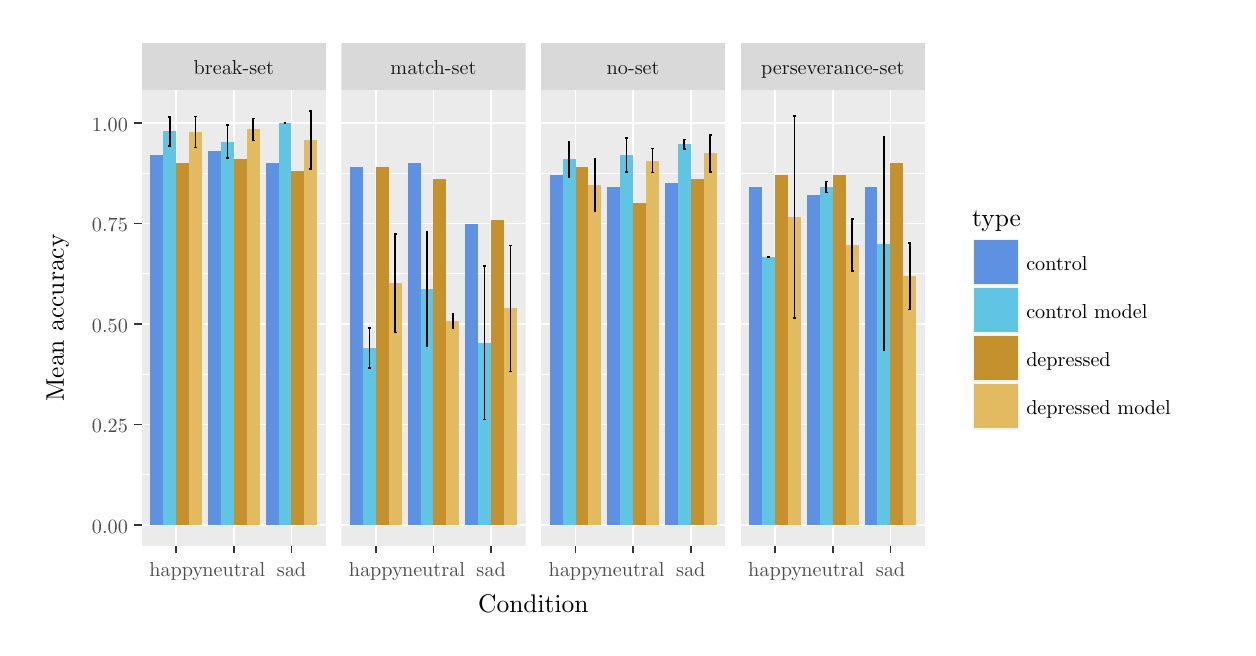
\begin{tikzpicture}[x=1pt,y=1pt]
\definecolor{fillColor}{RGB}{255,255,255}
\path[use as bounding box,fill=fillColor,fill opacity=0.00] (0,0) rectangle (433.62,216.81);
\begin{scope}
\path[clip] (  0.00,  0.00) rectangle (433.62,216.81);
\definecolor{drawColor}{RGB}{255,255,255}
\definecolor{fillColor}{RGB}{255,255,255}

\path[draw=drawColor,line width= 0.6pt,line join=round,line cap=round,fill=fillColor] (  0.00,  0.00) rectangle (433.62,216.81);
\end{scope}
\begin{scope}
\path[clip] ( 41.17, 29.59) rectangle (107.82,194.25);
\definecolor{fillColor}{gray}{0.92}

\path[fill=fillColor] ( 41.17, 29.59) rectangle (107.82,194.25);
\definecolor{drawColor}{RGB}{255,255,255}

\path[draw=drawColor,line width= 0.3pt,line join=round] ( 41.17, 55.23) --
	(107.82, 55.23);

\path[draw=drawColor,line width= 0.3pt,line join=round] ( 41.17, 91.54) --
	(107.82, 91.54);

\path[draw=drawColor,line width= 0.3pt,line join=round] ( 41.17,127.86) --
	(107.82,127.86);

\path[draw=drawColor,line width= 0.3pt,line join=round] ( 41.17,164.18) --
	(107.82,164.18);

\path[draw=drawColor,line width= 0.6pt,line join=round] ( 41.17, 37.07) --
	(107.82, 37.07);

\path[draw=drawColor,line width= 0.6pt,line join=round] ( 41.17, 73.39) --
	(107.82, 73.39);

\path[draw=drawColor,line width= 0.6pt,line join=round] ( 41.17,109.70) --
	(107.82,109.70);

\path[draw=drawColor,line width= 0.6pt,line join=round] ( 41.17,146.02) --
	(107.82,146.02);

\path[draw=drawColor,line width= 0.6pt,line join=round] ( 41.17,182.33) --
	(107.82,182.33);

\path[draw=drawColor,line width= 0.6pt,line join=round] ( 53.67, 29.59) --
	( 53.67,194.25);

\path[draw=drawColor,line width= 0.6pt,line join=round] ( 74.50, 29.59) --
	( 74.50,194.25);

\path[draw=drawColor,line width= 0.6pt,line join=round] ( 95.32, 29.59) --
	( 95.32,194.25);
\definecolor{fillColor}{RGB}{226,186,95}

\path[fill=fillColor] ( 58.36, 37.07) rectangle ( 63.04,179.11);
\definecolor{fillColor}{RGB}{196,145,45}

\path[fill=fillColor] ( 53.67, 37.07) rectangle ( 58.36,167.81);
\definecolor{fillColor}{RGB}{95,197,226}

\path[fill=fillColor] ( 48.98, 37.07) rectangle ( 53.67,179.31);
\definecolor{fillColor}{RGB}{95,145,226}

\path[fill=fillColor] ( 44.30, 37.07) rectangle ( 48.98,170.71);
\definecolor{fillColor}{RGB}{226,186,95}

\path[fill=fillColor] ( 79.18, 37.07) rectangle ( 83.87,180.03);
\definecolor{fillColor}{RGB}{196,145,45}

\path[fill=fillColor] ( 74.50, 37.07) rectangle ( 79.18,169.26);
\definecolor{fillColor}{RGB}{95,197,226}

\path[fill=fillColor] ( 69.81, 37.07) rectangle ( 74.50,175.58);
\definecolor{fillColor}{RGB}{95,145,226}

\path[fill=fillColor] ( 65.12, 37.07) rectangle ( 69.81,172.17);
\definecolor{fillColor}{RGB}{226,186,95}

\path[fill=fillColor] (100.01, 37.07) rectangle (104.69,176.28);
\definecolor{fillColor}{RGB}{196,145,45}

\path[fill=fillColor] ( 95.32, 37.07) rectangle (100.01,164.90);
\definecolor{fillColor}{RGB}{95,197,226}

\path[fill=fillColor] ( 90.64, 37.07) rectangle ( 95.32,182.33);
\definecolor{fillColor}{RGB}{95,145,226}

\path[fill=fillColor] ( 85.95, 37.07) rectangle ( 90.64,167.81);
\definecolor{drawColor}{RGB}{0,0,0}

\path[draw=drawColor,line width= 0.6pt,line join=round] ( 60.18,184.70) --
	( 61.22,184.70);

\path[draw=drawColor,line width= 0.6pt,line join=round] ( 60.70,184.70) --
	( 60.70,173.51);

\path[draw=drawColor,line width= 0.6pt,line join=round] ( 60.18,173.51) --
	( 61.22,173.51);

\path[draw=drawColor,line width= 0.6pt,line join=round] ( 50.81,184.55) --
	( 51.85,184.55);

\path[draw=drawColor,line width= 0.6pt,line join=round] ( 51.33,184.55) --
	( 51.33,174.07);

\path[draw=drawColor,line width= 0.6pt,line join=round] ( 50.81,174.07) --
	( 51.85,174.07);

\path[draw=drawColor,line width= 0.6pt,line join=round] ( 81.00,184.02) --
	( 82.05,184.02);

\path[draw=drawColor,line width= 0.6pt,line join=round] ( 81.52,184.02) --
	( 81.52,176.03);

\path[draw=drawColor,line width= 0.6pt,line join=round] ( 81.00,176.03) --
	( 82.05,176.03);

\path[draw=drawColor,line width= 0.6pt,line join=round] ( 71.63,181.52) --
	( 72.67,181.52);

\path[draw=drawColor,line width= 0.6pt,line join=round] ( 72.15,181.52) --
	( 72.15,169.64);

\path[draw=drawColor,line width= 0.6pt,line join=round] ( 71.63,169.64) --
	( 72.67,169.64);

\path[draw=drawColor,line width= 0.6pt,line join=round] (101.83,186.76) --
	(102.87,186.76);

\path[draw=drawColor,line width= 0.6pt,line join=round] (102.35,186.76) --
	(102.35,165.80);

\path[draw=drawColor,line width= 0.6pt,line join=round] (101.83,165.80) --
	(102.87,165.80);

\path[draw=drawColor,line width= 0.6pt,line join=round] ( 92.46,182.33) --
	( 93.50,182.33);

\path[draw=drawColor,line width= 0.6pt,line join=round] ( 92.98,182.33) --
	( 92.98,182.33);

\path[draw=drawColor,line width= 0.6pt,line join=round] ( 92.46,182.33) --
	( 93.50,182.33);
\end{scope}
\begin{scope}
\path[clip] (113.32, 29.59) rectangle (179.96,194.25);
\definecolor{fillColor}{gray}{0.92}

\path[fill=fillColor] (113.32, 29.59) rectangle (179.96,194.25);
\definecolor{drawColor}{RGB}{255,255,255}

\path[draw=drawColor,line width= 0.3pt,line join=round] (113.32, 55.23) --
	(179.96, 55.23);

\path[draw=drawColor,line width= 0.3pt,line join=round] (113.32, 91.54) --
	(179.96, 91.54);

\path[draw=drawColor,line width= 0.3pt,line join=round] (113.32,127.86) --
	(179.96,127.86);

\path[draw=drawColor,line width= 0.3pt,line join=round] (113.32,164.18) --
	(179.96,164.18);

\path[draw=drawColor,line width= 0.6pt,line join=round] (113.32, 37.07) --
	(179.96, 37.07);

\path[draw=drawColor,line width= 0.6pt,line join=round] (113.32, 73.39) --
	(179.96, 73.39);

\path[draw=drawColor,line width= 0.6pt,line join=round] (113.32,109.70) --
	(179.96,109.70);

\path[draw=drawColor,line width= 0.6pt,line join=round] (113.32,146.02) --
	(179.96,146.02);

\path[draw=drawColor,line width= 0.6pt,line join=round] (113.32,182.33) --
	(179.96,182.33);

\path[draw=drawColor,line width= 0.6pt,line join=round] (125.81, 29.59) --
	(125.81,194.25);

\path[draw=drawColor,line width= 0.6pt,line join=round] (146.64, 29.59) --
	(146.64,194.25);

\path[draw=drawColor,line width= 0.6pt,line join=round] (167.47, 29.59) --
	(167.47,194.25);
\definecolor{fillColor}{RGB}{226,186,95}

\path[fill=fillColor] (130.50, 37.07) rectangle (135.19,124.49);
\definecolor{fillColor}{RGB}{196,145,45}

\path[fill=fillColor] (125.81, 37.07) rectangle (130.50,166.36);
\definecolor{fillColor}{RGB}{95,197,226}

\path[fill=fillColor] (121.13, 37.07) rectangle (125.81,101.00);
\definecolor{fillColor}{RGB}{95,145,226}

\path[fill=fillColor] (116.44, 37.07) rectangle (121.13,166.36);
\definecolor{fillColor}{RGB}{226,186,95}

\path[fill=fillColor] (151.33, 37.07) rectangle (156.01,110.76);
\definecolor{fillColor}{RGB}{196,145,45}

\path[fill=fillColor] (146.64, 37.07) rectangle (151.33,162.00);
\definecolor{fillColor}{RGB}{95,197,226}

\path[fill=fillColor] (141.95, 37.07) rectangle (146.64,122.36);
\definecolor{fillColor}{RGB}{95,145,226}

\path[fill=fillColor] (137.27, 37.07) rectangle (141.95,167.81);
\definecolor{fillColor}{RGB}{226,186,95}

\path[fill=fillColor] (172.15, 37.07) rectangle (176.84,115.34);
\definecolor{fillColor}{RGB}{196,145,45}

\path[fill=fillColor] (167.47, 37.07) rectangle (172.15,147.47);
\definecolor{fillColor}{RGB}{95,197,226}

\path[fill=fillColor] (162.78, 37.07) rectangle (167.47,102.99);
\definecolor{fillColor}{RGB}{95,145,226}

\path[fill=fillColor] (158.10, 37.07) rectangle (162.78,146.02);
\definecolor{drawColor}{RGB}{0,0,0}

\path[draw=drawColor,line width= 0.6pt,line join=round] (132.32,142.27) --
	(133.36,142.27);

\path[draw=drawColor,line width= 0.6pt,line join=round] (132.84,142.27) --
	(132.84,106.70);

\path[draw=drawColor,line width= 0.6pt,line join=round] (132.32,106.70) --
	(133.36,106.70);

\path[draw=drawColor,line width= 0.6pt,line join=round] (122.95,108.17) --
	(123.99,108.17);

\path[draw=drawColor,line width= 0.6pt,line join=round] (123.47,108.17) --
	(123.47, 93.82);

\path[draw=drawColor,line width= 0.6pt,line join=round] (122.95, 93.82) --
	(123.99, 93.82);

\path[draw=drawColor,line width= 0.6pt,line join=round] (153.15,113.29) --
	(154.19,113.29);

\path[draw=drawColor,line width= 0.6pt,line join=round] (153.67,113.29) --
	(153.67,108.23);

\path[draw=drawColor,line width= 0.6pt,line join=round] (153.15,108.23) --
	(154.19,108.23);

\path[draw=drawColor,line width= 0.6pt,line join=round] (143.78,143.16) --
	(144.82,143.16);

\path[draw=drawColor,line width= 0.6pt,line join=round] (144.30,143.16) --
	(144.30,101.56);

\path[draw=drawColor,line width= 0.6pt,line join=round] (143.78,101.56) --
	(144.82,101.56);

\path[draw=drawColor,line width= 0.6pt,line join=round] (173.98,138.10) --
	(175.02,138.10);

\path[draw=drawColor,line width= 0.6pt,line join=round] (174.50,138.10) --
	(174.50, 92.59);

\path[draw=drawColor,line width= 0.6pt,line join=round] (173.98, 92.59) --
	(175.02, 92.59);

\path[draw=drawColor,line width= 0.6pt,line join=round] (164.60,130.72) --
	(165.64,130.72);

\path[draw=drawColor,line width= 0.6pt,line join=round] (165.12,130.72) --
	(165.12, 75.25);

\path[draw=drawColor,line width= 0.6pt,line join=round] (164.60, 75.25) --
	(165.64, 75.25);
\end{scope}
\begin{scope}
\path[clip] (185.46, 29.59) rectangle (252.11,194.25);
\definecolor{fillColor}{gray}{0.92}

\path[fill=fillColor] (185.46, 29.59) rectangle (252.11,194.25);
\definecolor{drawColor}{RGB}{255,255,255}

\path[draw=drawColor,line width= 0.3pt,line join=round] (185.46, 55.23) --
	(252.11, 55.23);

\path[draw=drawColor,line width= 0.3pt,line join=round] (185.46, 91.54) --
	(252.11, 91.54);

\path[draw=drawColor,line width= 0.3pt,line join=round] (185.46,127.86) --
	(252.11,127.86);

\path[draw=drawColor,line width= 0.3pt,line join=round] (185.46,164.18) --
	(252.11,164.18);

\path[draw=drawColor,line width= 0.6pt,line join=round] (185.46, 37.07) --
	(252.11, 37.07);

\path[draw=drawColor,line width= 0.6pt,line join=round] (185.46, 73.39) --
	(252.11, 73.39);

\path[draw=drawColor,line width= 0.6pt,line join=round] (185.46,109.70) --
	(252.11,109.70);

\path[draw=drawColor,line width= 0.6pt,line join=round] (185.46,146.02) --
	(252.11,146.02);

\path[draw=drawColor,line width= 0.6pt,line join=round] (185.46,182.33) --
	(252.11,182.33);

\path[draw=drawColor,line width= 0.6pt,line join=round] (197.96, 29.59) --
	(197.96,194.25);

\path[draw=drawColor,line width= 0.6pt,line join=round] (218.79, 29.59) --
	(218.79,194.25);

\path[draw=drawColor,line width= 0.6pt,line join=round] (239.61, 29.59) --
	(239.61,194.25);
\definecolor{fillColor}{RGB}{226,186,95}

\path[fill=fillColor] (202.64, 37.07) rectangle (207.33,159.99);
\definecolor{fillColor}{RGB}{196,145,45}

\path[fill=fillColor] (197.96, 37.07) rectangle (202.64,166.36);
\definecolor{fillColor}{RGB}{95,197,226}

\path[fill=fillColor] (193.27, 37.07) rectangle (197.96,169.21);
\definecolor{fillColor}{RGB}{95,145,226}

\path[fill=fillColor] (188.59, 37.07) rectangle (193.27,163.45);
\definecolor{fillColor}{RGB}{226,186,95}

\path[fill=fillColor] (223.47, 37.07) rectangle (228.16,168.80);
\definecolor{fillColor}{RGB}{196,145,45}

\path[fill=fillColor] (218.79, 37.07) rectangle (223.47,153.28);
\definecolor{fillColor}{RGB}{95,197,226}

\path[fill=fillColor] (214.10, 37.07) rectangle (218.79,170.76);
\definecolor{fillColor}{RGB}{95,145,226}

\path[fill=fillColor] (209.41, 37.07) rectangle (214.10,159.09);
\definecolor{fillColor}{RGB}{226,186,95}

\path[fill=fillColor] (244.30, 37.07) rectangle (248.98,171.35);
\definecolor{fillColor}{RGB}{196,145,45}

\path[fill=fillColor] (239.61, 37.07) rectangle (244.30,162.00);
\definecolor{fillColor}{RGB}{95,197,226}

\path[fill=fillColor] (234.93, 37.07) rectangle (239.61,174.65);
\definecolor{fillColor}{RGB}{95,145,226}

\path[fill=fillColor] (230.24, 37.07) rectangle (234.93,160.54);
\definecolor{drawColor}{RGB}{0,0,0}

\path[draw=drawColor,line width= 0.6pt,line join=round] (204.47,169.43) --
	(205.51,169.43);

\path[draw=drawColor,line width= 0.6pt,line join=round] (204.99,169.43) --
	(204.99,150.54);

\path[draw=drawColor,line width= 0.6pt,line join=round] (204.47,150.54) --
	(205.51,150.54);

\path[draw=drawColor,line width= 0.6pt,line join=round] (195.10,175.60) --
	(196.14,175.60);

\path[draw=drawColor,line width= 0.6pt,line join=round] (195.62,175.60) --
	(195.62,162.81);

\path[draw=drawColor,line width= 0.6pt,line join=round] (195.10,162.81) --
	(196.14,162.81);

\path[draw=drawColor,line width= 0.6pt,line join=round] (225.29,173.16) --
	(226.34,173.16);

\path[draw=drawColor,line width= 0.6pt,line join=round] (225.81,173.16) --
	(225.81,164.44);

\path[draw=drawColor,line width= 0.6pt,line join=round] (225.29,164.44) --
	(226.34,164.44);

\path[draw=drawColor,line width= 0.6pt,line join=round] (215.92,176.93) --
	(216.96,176.93);

\path[draw=drawColor,line width= 0.6pt,line join=round] (216.44,176.93) --
	(216.44,164.59);

\path[draw=drawColor,line width= 0.6pt,line join=round] (215.92,164.59) --
	(216.96,164.59);

\path[draw=drawColor,line width= 0.6pt,line join=round] (246.12,178.04) --
	(247.16,178.04);

\path[draw=drawColor,line width= 0.6pt,line join=round] (246.64,178.04) --
	(246.64,164.65);

\path[draw=drawColor,line width= 0.6pt,line join=round] (246.12,164.65) --
	(247.16,164.65);

\path[draw=drawColor,line width= 0.6pt,line join=round] (236.75,176.39) --
	(237.79,176.39);

\path[draw=drawColor,line width= 0.6pt,line join=round] (237.27,176.39) --
	(237.27,172.92);

\path[draw=drawColor,line width= 0.6pt,line join=round] (236.75,172.92) --
	(237.79,172.92);
\end{scope}
\begin{scope}
\path[clip] (257.61, 29.59) rectangle (324.25,194.25);
\definecolor{fillColor}{gray}{0.92}

\path[fill=fillColor] (257.61, 29.59) rectangle (324.25,194.25);
\definecolor{drawColor}{RGB}{255,255,255}

\path[draw=drawColor,line width= 0.3pt,line join=round] (257.61, 55.23) --
	(324.25, 55.23);

\path[draw=drawColor,line width= 0.3pt,line join=round] (257.61, 91.54) --
	(324.25, 91.54);

\path[draw=drawColor,line width= 0.3pt,line join=round] (257.61,127.86) --
	(324.25,127.86);

\path[draw=drawColor,line width= 0.3pt,line join=round] (257.61,164.18) --
	(324.25,164.18);

\path[draw=drawColor,line width= 0.6pt,line join=round] (257.61, 37.07) --
	(324.25, 37.07);

\path[draw=drawColor,line width= 0.6pt,line join=round] (257.61, 73.39) --
	(324.25, 73.39);

\path[draw=drawColor,line width= 0.6pt,line join=round] (257.61,109.70) --
	(324.25,109.70);

\path[draw=drawColor,line width= 0.6pt,line join=round] (257.61,146.02) --
	(324.25,146.02);

\path[draw=drawColor,line width= 0.6pt,line join=round] (257.61,182.33) --
	(324.25,182.33);

\path[draw=drawColor,line width= 0.6pt,line join=round] (270.10, 29.59) --
	(270.10,194.25);

\path[draw=drawColor,line width= 0.6pt,line join=round] (290.93, 29.59) --
	(290.93,194.25);

\path[draw=drawColor,line width= 0.6pt,line join=round] (311.76, 29.59) --
	(311.76,194.25);
\definecolor{fillColor}{RGB}{226,186,95}

\path[fill=fillColor] (274.79, 37.07) rectangle (279.48,148.44);
\definecolor{fillColor}{RGB}{196,145,45}

\path[fill=fillColor] (270.10, 37.07) rectangle (274.79,163.45);
\definecolor{fillColor}{RGB}{95,197,226}

\path[fill=fillColor] (265.42, 37.07) rectangle (270.10,133.91);
\definecolor{fillColor}{RGB}{95,145,226}

\path[fill=fillColor] (260.73, 37.07) rectangle (265.42,159.09);
\definecolor{fillColor}{RGB}{226,186,95}

\path[fill=fillColor] (295.62, 37.07) rectangle (300.30,138.24);
\definecolor{fillColor}{RGB}{196,145,45}

\path[fill=fillColor] (290.93, 37.07) rectangle (295.62,163.45);
\definecolor{fillColor}{RGB}{95,197,226}

\path[fill=fillColor] (286.24, 37.07) rectangle (290.93,159.28);
\definecolor{fillColor}{RGB}{95,145,226}

\path[fill=fillColor] (281.56, 37.07) rectangle (286.24,156.19);
\definecolor{fillColor}{RGB}{226,186,95}

\path[fill=fillColor] (316.44, 37.07) rectangle (321.13,127.00);
\definecolor{fillColor}{RGB}{196,145,45}

\path[fill=fillColor] (311.76, 37.07) rectangle (316.44,167.81);
\definecolor{fillColor}{RGB}{95,197,226}

\path[fill=fillColor] (307.07, 37.07) rectangle (311.76,138.76);
\definecolor{fillColor}{RGB}{95,145,226}

\path[fill=fillColor] (302.39, 37.07) rectangle (307.07,159.09);
\definecolor{drawColor}{RGB}{0,0,0}

\path[draw=drawColor,line width= 0.6pt,line join=round] (276.61,185.00) --
	(277.65,185.00);

\path[draw=drawColor,line width= 0.6pt,line join=round] (277.13,185.00) --
	(277.13,111.88);

\path[draw=drawColor,line width= 0.6pt,line join=round] (276.61,111.88) --
	(277.65,111.88);

\path[draw=drawColor,line width= 0.6pt,line join=round] (267.24,133.91) --
	(268.28,133.91);

\path[draw=drawColor,line width= 0.6pt,line join=round] (267.76,133.91) --
	(267.76,133.91);

\path[draw=drawColor,line width= 0.6pt,line join=round] (267.24,133.91) --
	(268.28,133.91);

\path[draw=drawColor,line width= 0.6pt,line join=round] (297.44,147.59) --
	(298.48,147.59);

\path[draw=drawColor,line width= 0.6pt,line join=round] (297.96,147.59) --
	(297.96,128.88);

\path[draw=drawColor,line width= 0.6pt,line join=round] (297.44,128.88) --
	(298.48,128.88);

\path[draw=drawColor,line width= 0.6pt,line join=round] (288.07,161.27) --
	(289.11,161.27);

\path[draw=drawColor,line width= 0.6pt,line join=round] (288.59,161.27) --
	(288.59,157.28);

\path[draw=drawColor,line width= 0.6pt,line join=round] (288.07,157.28) --
	(289.11,157.28);

\path[draw=drawColor,line width= 0.6pt,line join=round] (318.27,138.98) --
	(319.31,138.98);

\path[draw=drawColor,line width= 0.6pt,line join=round] (318.79,138.98) --
	(318.79,115.01);

\path[draw=drawColor,line width= 0.6pt,line join=round] (318.27,115.01) --
	(319.31,115.01);

\path[draw=drawColor,line width= 0.6pt,line join=round] (308.89,177.19) --
	(309.93,177.19);

\path[draw=drawColor,line width= 0.6pt,line join=round] (309.41,177.19) --
	(309.41,100.32);

\path[draw=drawColor,line width= 0.6pt,line join=round] (308.89,100.32) --
	(309.93,100.32);
\end{scope}
\begin{scope}
\path[clip] ( 41.17,194.25) rectangle (107.82,211.31);
\definecolor{fillColor}{gray}{0.85}

\path[fill=fillColor] ( 41.17,194.25) rectangle (107.82,211.31);
\definecolor{drawColor}{gray}{0.10}

\node[text=drawColor,anchor=base,inner sep=0pt, outer sep=0pt, scale=  0.73] at ( 74.50,199.75) {break-set};
\end{scope}
\begin{scope}
\path[clip] (113.32,194.25) rectangle (179.96,211.31);
\definecolor{fillColor}{gray}{0.85}

\path[fill=fillColor] (113.32,194.25) rectangle (179.96,211.31);
\definecolor{drawColor}{gray}{0.10}

\node[text=drawColor,anchor=base,inner sep=0pt, outer sep=0pt, scale=  0.73] at (146.64,199.75) {match-set};
\end{scope}
\begin{scope}
\path[clip] (185.46,194.25) rectangle (252.11,211.31);
\definecolor{fillColor}{gray}{0.85}

\path[fill=fillColor] (185.46,194.25) rectangle (252.11,211.31);
\definecolor{drawColor}{gray}{0.10}

\node[text=drawColor,anchor=base,inner sep=0pt, outer sep=0pt, scale=  0.73] at (218.79,199.75) {no-set};
\end{scope}
\begin{scope}
\path[clip] (257.61,194.25) rectangle (324.25,211.31);
\definecolor{fillColor}{gray}{0.85}

\path[fill=fillColor] (257.61,194.25) rectangle (324.25,211.31);
\definecolor{drawColor}{gray}{0.10}

\node[text=drawColor,anchor=base,inner sep=0pt, outer sep=0pt, scale=  0.73] at (290.93,199.75) {perseverance-set};
\end{scope}
\begin{scope}
\path[clip] (  0.00,  0.00) rectangle (433.62,216.81);
\definecolor{drawColor}{gray}{0.20}

\path[draw=drawColor,line width= 0.6pt,line join=round] ( 53.67, 26.84) --
	( 53.67, 29.59);

\path[draw=drawColor,line width= 0.6pt,line join=round] ( 74.50, 26.84) --
	( 74.50, 29.59);

\path[draw=drawColor,line width= 0.6pt,line join=round] ( 95.32, 26.84) --
	( 95.32, 29.59);
\end{scope}
\begin{scope}
\path[clip] (  0.00,  0.00) rectangle (433.62,216.81);
\definecolor{drawColor}{gray}{0.30}

\node[text=drawColor,anchor=base,inner sep=0pt, outer sep=0pt, scale=  0.73] at ( 53.67, 18.58) {happy};

\node[text=drawColor,anchor=base,inner sep=0pt, outer sep=0pt, scale=  0.73] at ( 74.50, 18.58) {neutral};

\node[text=drawColor,anchor=base,inner sep=0pt, outer sep=0pt, scale=  0.73] at ( 95.32, 18.58) {sad};
\end{scope}
\begin{scope}
\path[clip] (  0.00,  0.00) rectangle (433.62,216.81);
\definecolor{drawColor}{gray}{0.20}

\path[draw=drawColor,line width= 0.6pt,line join=round] (125.81, 26.84) --
	(125.81, 29.59);

\path[draw=drawColor,line width= 0.6pt,line join=round] (146.64, 26.84) --
	(146.64, 29.59);

\path[draw=drawColor,line width= 0.6pt,line join=round] (167.47, 26.84) --
	(167.47, 29.59);
\end{scope}
\begin{scope}
\path[clip] (  0.00,  0.00) rectangle (433.62,216.81);
\definecolor{drawColor}{gray}{0.30}

\node[text=drawColor,anchor=base,inner sep=0pt, outer sep=0pt, scale=  0.73] at (125.81, 18.58) {happy};

\node[text=drawColor,anchor=base,inner sep=0pt, outer sep=0pt, scale=  0.73] at (146.64, 18.58) {neutral};

\node[text=drawColor,anchor=base,inner sep=0pt, outer sep=0pt, scale=  0.73] at (167.47, 18.58) {sad};
\end{scope}
\begin{scope}
\path[clip] (  0.00,  0.00) rectangle (433.62,216.81);
\definecolor{drawColor}{gray}{0.20}

\path[draw=drawColor,line width= 0.6pt,line join=round] (197.96, 26.84) --
	(197.96, 29.59);

\path[draw=drawColor,line width= 0.6pt,line join=round] (218.79, 26.84) --
	(218.79, 29.59);

\path[draw=drawColor,line width= 0.6pt,line join=round] (239.61, 26.84) --
	(239.61, 29.59);
\end{scope}
\begin{scope}
\path[clip] (  0.00,  0.00) rectangle (433.62,216.81);
\definecolor{drawColor}{gray}{0.30}

\node[text=drawColor,anchor=base,inner sep=0pt, outer sep=0pt, scale=  0.73] at (197.96, 18.58) {happy};

\node[text=drawColor,anchor=base,inner sep=0pt, outer sep=0pt, scale=  0.73] at (218.79, 18.58) {neutral};

\node[text=drawColor,anchor=base,inner sep=0pt, outer sep=0pt, scale=  0.73] at (239.61, 18.58) {sad};
\end{scope}
\begin{scope}
\path[clip] (  0.00,  0.00) rectangle (433.62,216.81);
\definecolor{drawColor}{gray}{0.20}

\path[draw=drawColor,line width= 0.6pt,line join=round] (270.10, 26.84) --
	(270.10, 29.59);

\path[draw=drawColor,line width= 0.6pt,line join=round] (290.93, 26.84) --
	(290.93, 29.59);

\path[draw=drawColor,line width= 0.6pt,line join=round] (311.76, 26.84) --
	(311.76, 29.59);
\end{scope}
\begin{scope}
\path[clip] (  0.00,  0.00) rectangle (433.62,216.81);
\definecolor{drawColor}{gray}{0.30}

\node[text=drawColor,anchor=base,inner sep=0pt, outer sep=0pt, scale=  0.73] at (270.10, 18.58) {happy};

\node[text=drawColor,anchor=base,inner sep=0pt, outer sep=0pt, scale=  0.73] at (290.93, 18.58) {neutral};

\node[text=drawColor,anchor=base,inner sep=0pt, outer sep=0pt, scale=  0.73] at (311.76, 18.58) {sad};
\end{scope}
\begin{scope}
\path[clip] (  0.00,  0.00) rectangle (433.62,216.81);
\definecolor{drawColor}{gray}{0.30}

\node[text=drawColor,anchor=base east,inner sep=0pt, outer sep=0pt, scale=  0.73] at ( 36.22, 34.04) {0.00};

\node[text=drawColor,anchor=base east,inner sep=0pt, outer sep=0pt, scale=  0.73] at ( 36.22, 70.36) {0.25};

\node[text=drawColor,anchor=base east,inner sep=0pt, outer sep=0pt, scale=  0.73] at ( 36.22,106.67) {0.50};

\node[text=drawColor,anchor=base east,inner sep=0pt, outer sep=0pt, scale=  0.73] at ( 36.22,142.99) {0.75};

\node[text=drawColor,anchor=base east,inner sep=0pt, outer sep=0pt, scale=  0.73] at ( 36.22,179.30) {1.00};
\end{scope}
\begin{scope}
\path[clip] (  0.00,  0.00) rectangle (433.62,216.81);
\definecolor{drawColor}{gray}{0.20}

\path[draw=drawColor,line width= 0.6pt,line join=round] ( 38.42, 37.07) --
	( 41.17, 37.07);

\path[draw=drawColor,line width= 0.6pt,line join=round] ( 38.42, 73.39) --
	( 41.17, 73.39);

\path[draw=drawColor,line width= 0.6pt,line join=round] ( 38.42,109.70) --
	( 41.17,109.70);

\path[draw=drawColor,line width= 0.6pt,line join=round] ( 38.42,146.02) --
	( 41.17,146.02);

\path[draw=drawColor,line width= 0.6pt,line join=round] ( 38.42,182.33) --
	( 41.17,182.33);
\end{scope}
\begin{scope}
\path[clip] (  0.00,  0.00) rectangle (433.62,216.81);
\definecolor{drawColor}{RGB}{0,0,0}

\node[text=drawColor,anchor=base,inner sep=0pt, outer sep=0pt, scale=  0.92] at (182.71,  5.50) {Condition};
\end{scope}
\begin{scope}
\path[clip] (  0.00,  0.00) rectangle (433.62,216.81);
\definecolor{drawColor}{RGB}{0,0,0}

\node[text=drawColor,rotate= 90.00,anchor=base,inner sep=0pt, outer sep=0pt, scale=  0.92] at ( 13.08,111.92) {Mean accuracy};
\end{scope}
\begin{scope}
\path[clip] (  0.00,  0.00) rectangle (433.62,216.81);
\definecolor{fillColor}{RGB}{255,255,255}

\path[fill=fillColor] (335.63, 65.58) rectangle (428.12,158.25);
\end{scope}
\begin{scope}
\path[clip] (  0.00,  0.00) rectangle (433.62,216.81);
\definecolor{drawColor}{RGB}{0,0,0}

\node[text=drawColor,anchor=base west,inner sep=0pt, outer sep=0pt, scale=  0.92] at (341.32,144.99) {type};
\end{scope}
\begin{scope}
\path[clip] (  0.00,  0.00) rectangle (433.62,216.81);
\definecolor{drawColor}{RGB}{255,255,255}
\definecolor{fillColor}{gray}{0.95}

\path[draw=drawColor,line width= 0.6pt,line join=round,line cap=round,fill=fillColor] (341.32,123.31) rectangle (358.67,140.65);
\end{scope}
\begin{scope}
\path[clip] (  0.00,  0.00) rectangle (433.62,216.81);
\definecolor{fillColor}{RGB}{95,145,226}

\path[fill=fillColor] (342.04,124.02) rectangle (357.96,139.94);
\end{scope}
\begin{scope}
\path[clip] (  0.00,  0.00) rectangle (433.62,216.81);
\definecolor{drawColor}{RGB}{255,255,255}
\definecolor{fillColor}{gray}{0.95}

\path[draw=drawColor,line width= 0.6pt,line join=round,line cap=round,fill=fillColor] (341.32,105.96) rectangle (358.67,123.31);
\end{scope}
\begin{scope}
\path[clip] (  0.00,  0.00) rectangle (433.62,216.81);
\definecolor{fillColor}{RGB}{95,197,226}

\path[fill=fillColor] (342.04,106.67) rectangle (357.96,122.60);
\end{scope}
\begin{scope}
\path[clip] (  0.00,  0.00) rectangle (433.62,216.81);
\definecolor{drawColor}{RGB}{255,255,255}
\definecolor{fillColor}{gray}{0.95}

\path[draw=drawColor,line width= 0.6pt,line join=round,line cap=round,fill=fillColor] (341.32, 88.62) rectangle (358.67,105.96);
\end{scope}
\begin{scope}
\path[clip] (  0.00,  0.00) rectangle (433.62,216.81);
\definecolor{fillColor}{RGB}{196,145,45}

\path[fill=fillColor] (342.04, 89.33) rectangle (357.96,105.25);
\end{scope}
\begin{scope}
\path[clip] (  0.00,  0.00) rectangle (433.62,216.81);
\definecolor{drawColor}{RGB}{255,255,255}
\definecolor{fillColor}{gray}{0.95}

\path[draw=drawColor,line width= 0.6pt,line join=round,line cap=round,fill=fillColor] (341.32, 71.27) rectangle (358.67, 88.62);
\end{scope}
\begin{scope}
\path[clip] (  0.00,  0.00) rectangle (433.62,216.81);
\definecolor{fillColor}{RGB}{226,186,95}

\path[fill=fillColor] (342.04, 71.98) rectangle (357.96, 87.91);
\end{scope}
\begin{scope}
\path[clip] (  0.00,  0.00) rectangle (433.62,216.81);
\definecolor{drawColor}{RGB}{0,0,0}

\node[text=drawColor,anchor=base west,inner sep=0pt, outer sep=0pt, scale=  0.73] at (360.84,128.95) {control};
\end{scope}
\begin{scope}
\path[clip] (  0.00,  0.00) rectangle (433.62,216.81);
\definecolor{drawColor}{RGB}{0,0,0}

\node[text=drawColor,anchor=base west,inner sep=0pt, outer sep=0pt, scale=  0.73] at (360.84,111.60) {control model};
\end{scope}
\begin{scope}
\path[clip] (  0.00,  0.00) rectangle (433.62,216.81);
\definecolor{drawColor}{RGB}{0,0,0}

\node[text=drawColor,anchor=base west,inner sep=0pt, outer sep=0pt, scale=  0.73] at (360.84, 94.26) {depressed};
\end{scope}
\begin{scope}
\path[clip] (  0.00,  0.00) rectangle (433.62,216.81);
\definecolor{drawColor}{RGB}{0,0,0}

\node[text=drawColor,anchor=base west,inner sep=0pt, outer sep=0pt, scale=  0.73] at (360.84, 76.91) {depressed model};
\end{scope}
\end{tikzpicture}
